\chapter{Opis projektnog zadatka}
		
		Cilj ovog projekta je razviti programsku podršku za stvaranje responzivne web aplikacije \textit{"True Blood"} koja omogućuje prikupljanje i objavljivanje podataka o prikupljenim dozama darivane krvi te općenito vođenje evidencije podataka za banke krvi.
		Ovaj projekt omogućio bi smanjenje vremena i znatno olakšanje obavljanje administracijskih poslova pri samoj djelatnosti prikupljanja krvi. Vođenje evidencije 'klasičnim' načinom u današnje vrijeme je skupo, sporo i neefikasno, a ovim projektom nestaje potreba za standardnom hrpom papira, što ujedno i smanjuje kompliciranost, potrebu za dodatnom radnom snagom te dodatne troškove, a da ne govorimo o mogućoj dodatnoj redundanciji podataka i njihovoj mogućoj većoj opsežnosti.\\
		
		Nelogiranom korisniku se na javim web stranicama prikazuje trenutno stanje zaliha različitih krvnih grupa te mogućnost logina i registracije. U sustavu postoje 3 vrste korisnika:
		\begin{packed_item}
			\item{administrator}
			\item{djelatnik banke}
			\item{donor}
		\end{packed_item}
		Svaki korisnik (osim administratora) na svoju email adresu dobiva link za aktivaciju korisničkog računa i donorID koji će koristiti kao korisničko ime. Prilikom aktivacije korisničkog računa korisnik odabire lozinku koju će koristiti.
		\underbar{ \textit{Administrator} }sustava administrira korisničke račune. On kreira nove korisničke račune za ulogu djelatnika banke (ili donora) te može u bilo kojem trenutku deaktivirati bilo koji korisnički račun. Administrator isto tako definira gornju i donju granicu optimalne količine krvi za svaku krvnu grupu, kako bi sustav dojavio upozorenja u slučaju prekoračenja gornje ili donje granice.
		\underbar{ \textit{Djelatnik banke} }krvi evidentira podatke o donoru kada potencijalni donor pristupa darivanju krvi. Ukoliko donor još nije evidentiran u sustavu, djelatnik banke kreira njegov korisnički profil te popunjava sve potrebne podatke:
		\begin{packed_item}
			\item{matični podaci}
			\item{kontakt podaci}
			\item{zdrastveni podaci}
		\end{packed_item}
		Ukoliko je donor već koristio usluge ustanove, povlače se zadnji aktualni podaci koje djelatnik banke po potrebi nadopunjuje. Djelatnik banke u sustav evidentira svaki pokušaj doniranja. Prije nego donor pristupi darivanju krvi, djelatnik banke provjerava njegovo zdrastveno stanje, te prema tome može prihvatiti te privremeno ili trajno odbiti donora.
		Djelatnik banke evidentira uspješno doniranje krvi, ali i potrošnju (tj. slanje određenog broja jedinica krvi van banke). Time se povećava tj. smanjuje zaliha određene krvne grupe što je odmah vidljivo na javim web stranicama, a ukoliko se prekorači gornja ili donja granica zalihe za neku krvnu grupu, djelatnici dobivaju notifikaciju putem emaila.
		\underbar{ \textit{Donori} }imaju mogućnost sami se registrirati na web stranici te ažurirati svoje matične i kontakt podatke te pregledavati zapisane zdrastvene podatke i povijest svojih (uspješnih i odbijenih) doniranja. Svakom evidencijom uspješnog darivanja krvi, donor na svoj email dobiva poruku s potvrdom o pristupanju darivanju krvi u PDF formatu koju može i sam podići naknadno iz aplikacije. Prilikom svakog logiranja donora u sustav (koji nema trajnu zabranu darivanja krvi), aplikacija će donoru prikazati poruku u ovisnosti o trenutnom stanju zaliha krvi za njegovu krvnu grupu:
		\begin{packed_item}
			\item{stanje zaliha je ispod optimalne granice}
			\item{stanje zaliha je optimalno}
			\item{stanje zaliha je iznad gornje optimalne granice}
		\end{packed_item}
		Donori dobivaju notifikacije od sustava nakon što istekne dopušteni period od zadnjeg darivanja i ukoliko zaliha njihove krvne grupe padne ispod minimalne granice.\\
		
		Ovo rješenje bi mogle koristiti jednako manje ali i veće banke krvi koje još nemaju informacijski sustav za prikupljanje i objavljivanje podataka o prikupljenim dozama krvi. Pošto se radi o web aplikaciji, ona se lako može implementirati u postojeći sustav web stranica koju pojedini potencijalni korisnik rješenja ima, te se, ukoliko je to zbilja potrebno, i stil same web aplikacije može prilagoditi da korespondira sa stilom postojećih web stranica. Isto tako, ukoliko potencijalni korisnik već posjeduje neku vlastitu bazu podataka koju koristi za neku funkcionalnost logiranja i/ili evidenciju nekih relativnih podataka te bi ju htio nastaviti koristiti, rješenje je moguće prilagoditi da se koristi zahtijevanim podacima.\\
		
		Trenutno u hrvatskoj postoje implementirani dijelovi ovih rješenja, točnije, postoje javne stranice gdje se prikazuje trenutno stanje zaliha različitih krvnih grupa (npr. slika \ref{fig:HZTMprimjer}). Ako pogledamo malo šire po svijetu, možemo uočiti da ima očito i nekih razrađenih sistema za evidenciju sa loginom donora (npr. slika \ref{fig:AmericanRedCrossPrimjer}), no sva ta rješenja nemaju kompaktno razrađen sustav kod kojih bi prijašnji donori dobivali notifikacije s obzirom na stanje banke krvi i pojedinačnih krvnih grupa, koje je javno i na jednostavan (grafički) način dostupno svima.
		\begin{figure}[H]
			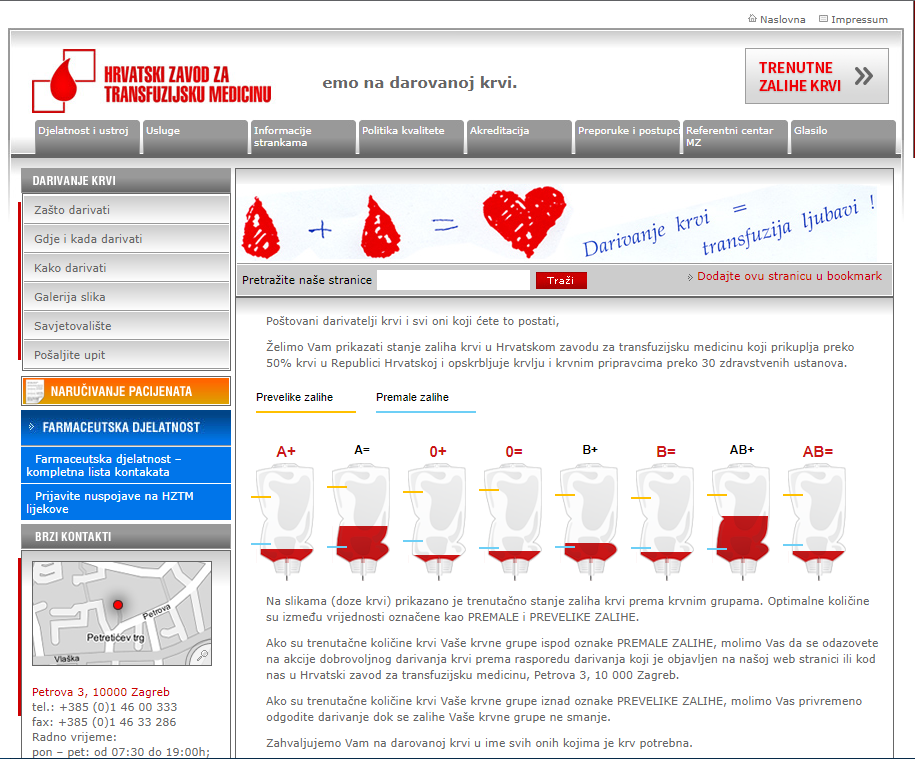
\includegraphics[scale=0.4]{slike/HZTMprimjer.PNG} %veličina slike u odnosu na originalnu datoteku i pozicija slike
			\centering
			\caption{Primjer javno dostupnih podataka o stanju banke krvi Hrvatskog zavoda za transfuzijsku medicinu}
			\label{fig:HZTMprimjer}
		\end{figure}
		\begin{figure}[H]
			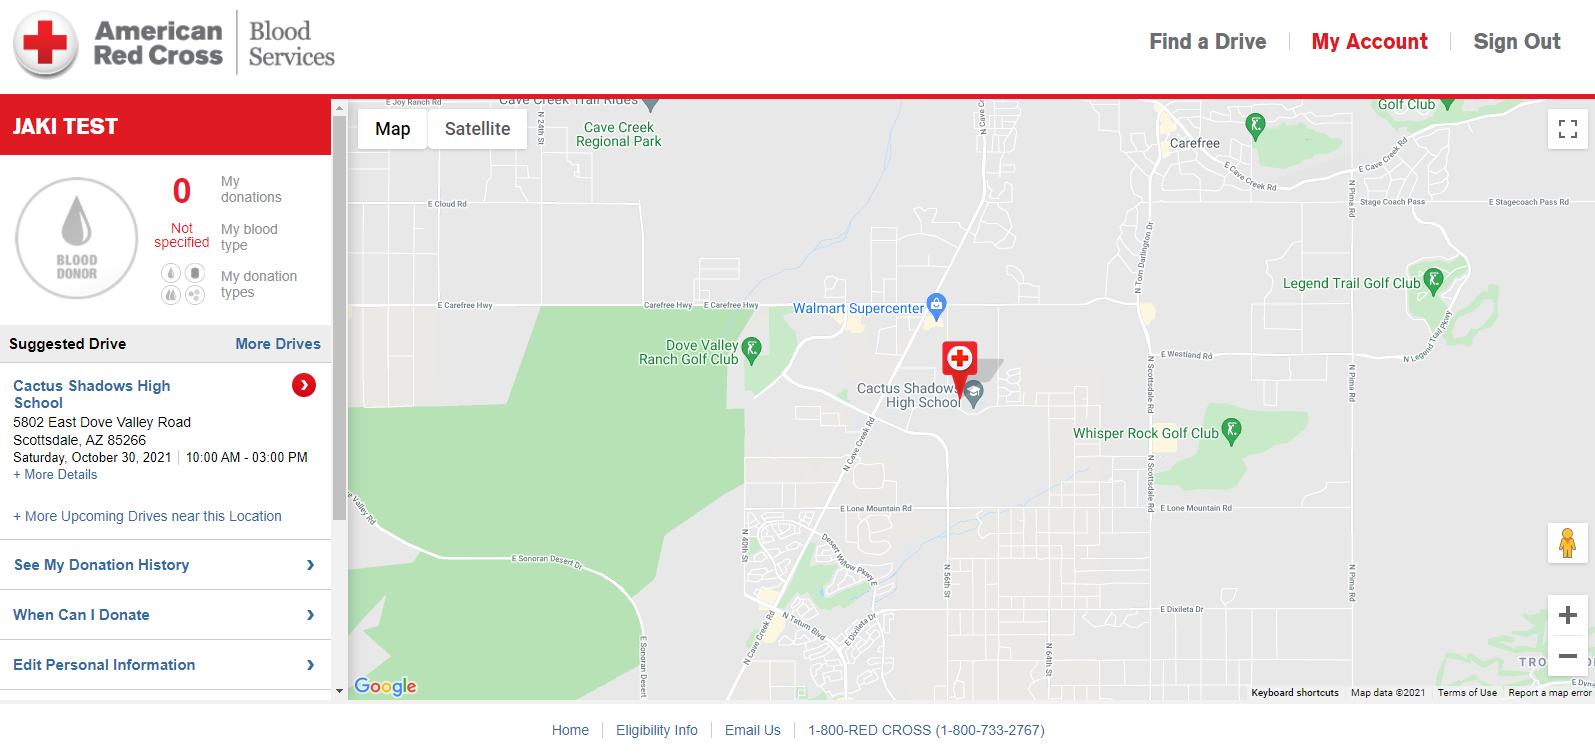
\includegraphics[scale=0.4]{slike/AmericanRedCrossPrimjer.PNG} %veličina slike u odnosu na originalnu datoteku i pozicija slike
			\centering
			\caption{Primjer web sučelja logiranog korisnika Američkog crvenog križa}
			\label{fig:AmericanRedCrossPrimjer}
		\end{figure}
\eject
		Ovo rješenje ima i nešto mjesta za kasniju nadogradnju. Jedna od mogućnosti je ugradnja podrške za notifikacije putem SMS poruka. Moguće je kasnije dodavanje i nešto poput nagradnog sistema za donore gdje bi donori svakim darivanjem krvi skupljali bodove koje bi mogli iskoristiti npr. za neke popuste kod nekih sponzora, besplatan ručak, ulaznicu u kino itd. 
		Naravno, kasnijih nadogradnji (i samih prilagodbi) može biti još, ovisno o željama i kasnijim potrebama korisnika rješenja, ukoliko su izvediva u sklopu ovog projekta.
		\eject
